%%%%%%%%%%%%%%%%%%%%%%%%%%%%%%%%%%%%%%%%%%%%%%%%%%%%%%%%%%%%%%%%%%%%%%%%%%%%%%%%%%
\begin{frame}[fragile]\frametitle{}
\begin{center}
{\Large Jottings from Talks, Tweets}

{\small Naval Ravikant}


\end{center}
\end{frame}


%%%%%%%%%%%%%%%%%%%%%%%%%%%%%%%%%%%%%%%%%%%%%%%%%%%%%%%%%%%
\begin{frame}[fragile]\frametitle{Stress}

	\begin{itemize}
	\item Stress happens when something wants to be in two places at one time. Like iron rod getting pulled from two ends.
	\item Stress is an inability to decide what’s important
	\item You want to find peace from mind. 
	\end{itemize}

\end{frame}

%%%%%%%%%%%%%%%%%%%%%%%%%%%%%%%%%%%%%%%%%%%%%%%%%%%%%%%%%%%
\begin{frame}[fragile]\frametitle{Peace}

	\begin{itemize}
	\item Peace is happiness at rest.
	\item Happiness is Peace in motion.
	\item The ultimate goal is not happiness, even though we use that term a lot. The goal is peace.
	\end{itemize}

\end{frame}

%%%%%%%%%%%%%%%%%%%%%%%%%%%%%%%%%%%%%%%%%%%%%%%%%%%%%%%%%%%
\begin{frame}[fragile]\frametitle{How do you get to peace?}

	\begin{itemize}
	\item Fundamentally, peace is inactivity; it’s a sense that everything is fine.
	\item If everything is fine, you’re not doing any physical or mental activity to change it. 
	\item You’re also not wishing you were doing something to change it, because that creates stress. 
	\end{itemize}

\end{frame}

%%%%%%%%%%%%%%%%%%%%%%%%%%%%%%%%%%%%%%%%%%%%%%%%%%%%%%%%%%%
\begin{frame}[fragile]\frametitle{How do you get to peace?}

	\begin{itemize}
	\item You cannot work toward peace, only understanding
	\item ``The name of God is truth.''
	\item If/once you understand true nature of everything, then you are at Peace.
	\end{itemize}

\end{frame}

%%%%%%%%%%%%%%%%%%%%%%%%%%%%%%%%%%%%%%%%%%%%%%%%%%%%%%%%%%%
\begin{frame}[fragile]\frametitle{Meditation}

	\begin{itemize}

	\item Free mind associates with things it sees, then imagines
	\item Contemplating on a subject, various aspects related to them
	\item Concentration is focusing on a topic
	\item Most meditation techniques are of concentration with a hope that at one stage you will be free from the concentration subject. 
	\item Meditation is actually beyond concentration. 
	\item You cannot do meditation. It happens when you are not doing anything. 
	\item Be still 1 hr a day. On one day you will reach a state where no thoughts bubble up.
	\end{itemize}

\end{frame}

%%%%%%%%%%%%%%%%%%%%%%%%%%%%%%%%%%%%%%%%%%%%%%%%%%%%%%%%%%%
\begin{frame}[fragile]\frametitle{Life Formulas}

	\begin{itemize}

	\item Happiness = Health + Wealth + Good Relationships 
\item Health = Exercise + Diet + Sleep 
\item Exercise = High Intensity Resistance Training + Sports + Rest 
\item Diet = Natural Foods + Intermittent Fasting + Plants 
\item Sleep = No alarms + 8–9 hours + Circadian rhythms 
\item Wealth = Income + Wealth * (Return on Investment) 
\item Income = Accountability + Leverage + Specific Knowledge 
\item Accountability = Personal Branding + Personal Platform + Taking Risk? 
\item Leverage = Capital + People + Intellectual Property 
\item Specific Knowledge = Knowing how to do something society cannot yet easily train other people to do 
\item Return on Investment = ``Buy-and-Hold'' + Valuation + Margin of Safety
	\end{itemize}

\end{frame}

%%%%%%%%%%%%%%%%%%%%%%%%%%%%%%%%%%%%%%%%%%%%%%%%%%%%%%%%%%%
\begin{frame}[fragile]\frametitle{Life Rules}

	\begin{itemize}
\item Be present above all else. 
\item Desire is suffering. (Buddha) 
\item Anger is a hot coal you hold in your hand while waiting to throw it at someone else. (Buddha) 
\item If you can't see yourself working with someone for life, don't work with them for a day. 
\item Reading (learning) is the ultimate meta-skill and can be traded for anything else. 
\item All the real benefits in life come from compound interest. 
\item Earn with your mind, not your time. 
\item 99 percent of all effort is wasted. 
\item Total honesty at all times. It's almost always possible to be honest and positive. 
\item Praise specifically, criticize generally. (Warren Buffett) 
\item Truth is that which has predictive power. 
\item Watch every thought. (Ask ``Why am I having this thought?'') 
\item All greatness comes from suffering. 
\item Love is given, not received. 
\item Enlightenment is the space between your thoughts. (Eckhart Tolle) 
\item Mathematics is the language of nature. 
\item Every moment has to be complete in and of itself.
	\end{itemize}

\end{frame}


%%%%%%%%%%%%%%%%%%%%%%%%%%%%%%%%%%%%%%%%%%%%%%%%%%%%%%%%%%%
\begin{frame}[fragile]\frametitle{Life Playbook}

Happiness = Health + Wealth + Good relationships
\begin{itemize}
\item Health = Exercise + Diet + Sleep
		\begin{itemize}
		\item Exercise = High Intensity Resistance training + Sports + Rest
		\item Diet = Natural Foods + Intermittent Fasting + Plants
		\item Sleep = No Alarms + 8-9 hours + Circadian Rhythms
		\end{itemize}

\item Wealth = Income + RoI
		\begin{itemize}
		\item Income = Accountability + Leverage + Specific Knowledge
			\begin{itemize}
			\item Accountability = Personal Branding + Personal Platform + Taking Risk
			\item Leverage = Capital + People + Intellectual Property
			\item Specific Knowledge =  Knowing how to do something that society cannot yet easily train other people to do
			\end{itemize}
		\item RoI = Buy-and-Hold + Valuation + Margin of Safety
		\end{itemize}
\end{itemize}


\end{frame}

%%%%%%%%%%%%%%%%%%%%%%%%%%%%%%%%%%%%%%%%%%%%%%%%%%%%%%%%%%%
\begin{frame}[fragile]\frametitle{Life Play-book Summary}

\begin{itemize}
\item Fast, lift, sprint, stretch, and meditate.
\item Build, sell, write, create, invest, and own.
\item Read, reflect, love, seek truth, and ignore society.
\item Make these habits. Say no to everything else.
\item Avoid debt, jail, addiction, disgrace, shortcuts, and media.
\item Relax. Victory is assured.
\end{itemize}

\end{frame}

%%%%%%%%%%%%%%%%%%%%%%%%%%%%%%%%%%%%%%%%%%%%%%%%%%%%%%%%%%%%%%%%%%%%%%%%%%%%%%%%%%
\begin{frame}[fragile]\frametitle{}
\begin{center}
{\Large Top 10 Life Learnings \ldots }

\end{center}
\end{frame}

%%%%%%%%%%%%%%%%%%%%%%%%%%%%%%%%%%%%%%%%%%%%%%%%%%%%%%%%%%%%%%%%%%%%%%%%%%%%%%%%%%
\begin{frame}[fragile]\frametitle{1}
\begin{center}
When looking for a purpose to life, notice that most things are stepping stones, done for ulterior motives.
\end{center}
\end{frame}

%%%%%%%%%%%%%%%%%%%%%%%%%%%%%%%%%%%%%%%%%%%%%%%%%%%%%%%%%%%%%%%%%%%%%%%%%%%%%%%%%%
\begin{frame}[fragile]\frametitle{2}
\begin{center}
If you ever want to have peace in your life, you have to move beyond good and evil.
\end{center}
\end{frame}

%%%%%%%%%%%%%%%%%%%%%%%%%%%%%%%%%%%%%%%%%%%%%%%%%%%%%%%%%%%%%%%%%%%%%%%%%%%%%%%%%%
\begin{frame}[fragile]\frametitle{3}
\begin{center}
 To measure the quality of your life, simply do nothing, and see how it feels.
\end{center}
\end{frame}

%%%%%%%%%%%%%%%%%%%%%%%%%%%%%%%%%%%%%%%%%%%%%%%%%%%%%%%%%%%%%%%%%%%%%%%%%%%%%%%%%%
\begin{frame}[fragile]\frametitle{4}
\begin{center}
No one can compete with you on being you. Most of life is a search for who and what needs you the most.
\end{center}
\end{frame}

%%%%%%%%%%%%%%%%%%%%%%%%%%%%%%%%%%%%%%%%%%%%%%%%%%%%%%%%%%%%%%%%%%%%%%%%%%%%%%%%%%
\begin{frame}[fragile]\frametitle{5}
\begin{center}
Living a life of integrity pays off, but it takes a very long time.
\end{center}
\end{frame}

%%%%%%%%%%%%%%%%%%%%%%%%%%%%%%%%%%%%%%%%%%%%%%%%%%%%%%%%%%%%%%%%%%%%%%%%%%%%%%%%%%
\begin{frame}[fragile]\frametitle{6}
\begin{center}
Three things in life: your health, your mission, and the people you love. That's it.\end{center}
\end{frame}

%%%%%%%%%%%%%%%%%%%%%%%%%%%%%%%%%%%%%%%%%%%%%%%%%%%%%%%%%%%%%%%%%%%%%%%%%%%%%%%%%%
\begin{frame}[fragile]\frametitle{7}
\begin{center}
Play iterated games. All the returns in life, whether in wealth, relationships, or knowledge, come from compound interest.
\end{center}
\end{frame}

%%%%%%%%%%%%%%%%%%%%%%%%%%%%%%%%%%%%%%%%%%%%%%%%%%%%%%%%%%%%%%%%%%%%%%%%%%%%%%%%%%
\begin{frame}[fragile]\frametitle{8}
\begin{center}
Religion, science, and spirituality help us make sense of the world. Life without at least one of them is a lonely and confusing place.
\end{center}
\end{frame}

%%%%%%%%%%%%%%%%%%%%%%%%%%%%%%%%%%%%%%%%%%%%%%%%%%%%%%%%%%%%%%%%%%%%%%%%%%%%%%%%%%
\begin{frame}[fragile]\frametitle{9}
\begin{center}
Life is a single-player game.
\end{center}
\end{frame}


%%%%%%%%%%%%%%%%%%%%%%%%%%%%%%%%%%%%%%%%%%%%%%%%%%%%%%%%%%%%%%%%%%%%%%%%%%%%%%%%%%
\begin{frame}[fragile]\frametitle{10}
\begin{center}
You can get almost anything you want out of life, as long as it's one thing and you want it far more than anything else.
\end{center}
\end{frame}


%%%%%%%%%%%%%%%%%%%%%%%%%%%%%%%%%%%%%%%%%%%%%%%%%%%%%%%%%%%%%%%%%%%%%%%%%%%%%%%%%%
\begin{frame}[fragile]\frametitle{Bonus}
\begin{center}
Of all the cards you can pick in the game of life, choose intelligence and drive. You can trade those two for almost anything else.
\end{center}
\end{frame}


%%%%%%%%%%%%%%%%%%%%%%%%%%%%%%%%%%%%%%%%%%%%%%%%%%%%%%%%%%%%%%%%%%%%%%%%%%%%%%%%%%
\begin{frame}[fragile]\frametitle{}
\begin{center}
{\Large Top 10 Meditation Learnings \ldots }

\end{center}
\end{frame}

%%%%%%%%%%%%%%%%%%%%%%%%%%%%%%%%%%%%%%%%%%%%%%%%%%%%%%%%%%%%%%%%%%%%%%%%%%%%%%%%%%
\begin{frame}[fragile]\frametitle{1}
\begin{center}
Meditation is not you going through thoughts - it’s letting thoughts go through you.
\end{center}
\end{frame}

%%%%%%%%%%%%%%%%%%%%%%%%%%%%%%%%%%%%%%%%%%%%%%%%%%%%%%%%%%%%%%%%%%%%%%%%%%%%%%%%%%
\begin{frame}[fragile]\frametitle{2}
\begin{center}
Yoga cultivates Peace of Body. Meditation cultivates Peace of Mind.
\end{center}
\end{frame}

%%%%%%%%%%%%%%%%%%%%%%%%%%%%%%%%%%%%%%%%%%%%%%%%%%%%%%%%%%%%%%%%%%%%%%%%%%%%%%%%%%
\begin{frame}[fragile]\frametitle{3}
\begin{center}
Meditation and transcendence are the birthrights of every human being..
\end{center}
\end{frame}

%%%%%%%%%%%%%%%%%%%%%%%%%%%%%%%%%%%%%%%%%%%%%%%%%%%%%%%%%%%%%%%%%%%%%%%%%%%%%%%%%%
\begin{frame}[fragile]\frametitle{4}
\begin{center}
Consider meditation as “self-therapy.” Instead of paying a therapist to listen to you, listen to yourself (non-judgmentally) until you accept or drop the fears.
\end{center}
\end{frame}

%%%%%%%%%%%%%%%%%%%%%%%%%%%%%%%%%%%%%%%%%%%%%%%%%%%%%%%%%%%%%%%%%%%%%%%%%%%%%%%%%%
\begin{frame}[fragile]\frametitle{5}
\begin{center}
Meditation, arts and artisan-ship, craftsmanship, politics, are other activities with learning curves detached from physical ability.
\end{center}
\end{frame}

%%%%%%%%%%%%%%%%%%%%%%%%%%%%%%%%%%%%%%%%%%%%%%%%%%%%%%%%%%%%%%%%%%%%%%%%%%%%%%%%%%
\begin{frame}[fragile]\frametitle{6}
\begin{center}
Meditation is turning off society and listening to yourself. It only “works” when done for its own sake.\end{center}
\end{frame}

%%%%%%%%%%%%%%%%%%%%%%%%%%%%%%%%%%%%%%%%%%%%%%%%%%%%%%%%%%%%%%%%%%%%%%%%%%%%%%%%%%
\begin{frame}[fragile]\frametitle{7}
\begin{center}
Insight meditation lets you run your brain in debug mode until you realize that you're just a subroutine in a larger program.
\end{center}
\end{frame}

%%%%%%%%%%%%%%%%%%%%%%%%%%%%%%%%%%%%%%%%%%%%%%%%%%%%%%%%%%%%%%%%%%%%%%%%%%%%%%%%%%
\begin{frame}[fragile]\frametitle{8}
\begin{center}
Perhaps one reason why yoga and meditation are hard to sustain is that they have no extrinsic value. Purely single-player games.
\end{center}
\end{frame}

%%%%%%%%%%%%%%%%%%%%%%%%%%%%%%%%%%%%%%%%%%%%%%%%%%%%%%%%%%%%%%%%%%%%%%%%%%%%%%%%%%
\begin{frame}[fragile]\frametitle{9}
\begin{center}
Meditation is intermittent fasting for the mind. Too much sugar leads to a heavy body, and too many distractions lead to a heavy mind.
\end{center}
\end{frame}


%%%%%%%%%%%%%%%%%%%%%%%%%%%%%%%%%%%%%%%%%%%%%%%%%%%%%%%%%%%%%%%%%%%%%%%%%%%%%%%%%%
\begin{frame}[fragile]\frametitle{10}
\begin{center}
If meditation was easy, you’d do nothing else.
\end{center}
\end{frame}


%%%%%%%%%%%%%%%%%%%%%%%%%%%%%%%%%%%%%%%%%%%%%%%%%%%%%%%%%%%
\begin{frame}[fragile]\frametitle{Goals vs Being Present}

\begin{itemize}
\item Goals: living in future, obligations, urge to do more and more
\item Being Present: less obligations, more natural, more productivity, better quality of work.
\end{itemize}

\end{frame}


%%%%%%%%%%%%%%%%%%%%%%%%%%%%%%%%%%%%%%%%%%%%%%%%%%%%%%%%%%%
\begin{frame}[fragile]\frametitle{How to get rich}

\begin{itemize}
\item There is no skill like Business.
\item Business cannot be learnt in school
\item What you really want is to figure out what Society wants and does not know how to get it yet. You need to provide that and that too, at scale.
\item Mostly dynamic, but if you have specific knowledge that you are passionate about, you can find matching desire from society. Or time brings it to your plate.
\item Need: Specific Knowledge, Accountability to own brand, Leverage/amplification
\end{itemize}

\end{frame}

%%%%%%%%%%%%%%%%%%%%%%%%%%%%%%%%%%%%%%%%%%%%%%%%%%%%%%%%%%%
\begin{frame}[fragile]\frametitle{Meaning of Life}

\begin{itemize}
\item Nonsense question.
\item One end goal leads to another and so on.
\item These are games, first marks, then education, then job, status, money, etc. Just games.
\item Living the life as it goes.
\end{itemize}

\end{frame}


%%%%%%%%%%%%%%%%%%%%%%%%%%%%%%%%%%%%%%%%%%%%%%%%%%%%%%%%%%%
\begin{frame}[fragile]\frametitle{Wealth vs Status}

\begin{itemize}
\item All of us want to be Free.
\item Easiest way to solve money problem by money. Be rich first.
\item Wealth positive sum game. Create more wealth without taking away from anyone.
\item Status is zero sum game. Only one can be number one at the cost of others.
\item Status guys attack Wealth as they cannot get it.
\end{itemize}

\end{frame}

%%%%%%%%%%%%%%%%%%%%%%%%%%%%%%%%%%%%%%%%%%%%%%%%%%%%%%%%%%%
\begin{frame}[fragile]\frametitle{What to look for in people}

\begin{itemize}
\item In Business: Intelligence, Energy, Integrity
\item In Relationships: Honesty, Calm (emotional self control)
\end{itemize}

\end{frame}

%%%%%%%%%%%%%%%%%%%%%%%%%%%%%%%%%%%%%%%%%%%%%%%%%%%%%%%%%%%
\begin{frame}[fragile]\frametitle{Philosophy book recommendation}

\begin{itemize}
\item For starters: Siddhartha, Herman Hess
\item For Advanced: Krishnamurthy Total Freedom, Osho Great Challenge, Marcus Meditations
\end{itemize}

\end{frame}

%%%%%%%%%%%%%%%%%%%%%%%%%%%%%%%%%%%%%%%%%%%%%%%%%%%%%%%%%%%
\begin{frame}[fragile]\frametitle{Modern Struggle}

\begin{itemize}
\item All our diseases are diseases of abundance in the modern times.
\item In old times, of scarcity, you consume whatever you get your hands laid on eg Sugar, News, etc for my survival
\item We are over exposed to everything. Brain can not cope up with that deluge. If you pay attention to all, it will drive you insane. 
\item Social media is addictive like Sugar.
\item Resist. 
\end{itemize}

\end{frame}











%%%%%%%%%%%%%%%%%%%%%%%%%%%%%%%%%%%%%%%%%%%%%%%%%%%%%%%%%%%
\begin{frame}[fragile]\frametitle{Farnam Street talk}

\begin{itemize}
\item My number one priority in life, above my happiness, above my family, above my work, is my own health.
\item I try and set up good systems and then the individual decisions don’t matter that matter much
\item Science is, to me, the study of truth. It is the only true discipline because it makes falsifiable predictions.
\end{itemize}

\end{frame}

%%%%%%%%%%%%%%%%%%%%%%%%%%%%%%%%%%%%%%%%%%%%%%%%%%%%%%%%%%%
\begin{frame}[fragile]\frametitle{Farnam Street talk}

\begin{itemize}
\item To me, happiness is not about positive thoughts. It’s not about negative thoughts. It’s about the absence of desire, especially the absence of desire for external things.
\item Happiness to me is mainly not suffering, not desiring, not thinking too much about the future or the past, really embracing the present moment and
the reality of what is, the way it is.
\end{itemize}

\end{frame}

%%%%%%%%%%%%%%%%%%%%%%%%%%%%%%%%%%%%%%%%%%%%%%%%%%%%%%%%%%%
\begin{frame}[fragile]\frametitle{Farnam Street talk}

\begin{itemize}
\item I don’t believe that I have the ability to say what is going to work. 
\item Rather, what I try to do is try to eliminate what’s not going to work. 
\item It’s not about having correct judgment. 
\item It’s about avoiding incorrect judgments.
\end{itemize}

\end{frame}

%%%%%%%%%%%%%%%%%%%%%%%%%%%%%%%%%%%%%%%%%%%%%%%%%%%%%%%%%%%
\begin{frame}[fragile]\frametitle{Farnam Street talk}

\begin{itemize}
\item I think all the benefits in life come from compound interest. 
\item I only want to be around people that I know I’m going to be around with for the rest of my life. 
\item I only want to work on things that I know have a long-term payout.
\item I think if you take a very long-term point of view and if you take the emotion out of it, then I wouldn’t consider those things mistakes anymore.
\end{itemize}

\end{frame}

%%%%%%%%%%%%%%%%%%%%%%%%%%%%%%%%%%%%%%%%%%%%%%%%%%%%%%%%%%%
\begin{frame}[fragile]\frametitle{Farnam Street talk}

\begin{itemize}
\item Macroeconomics is a combination of voodoo complex systems and politics. 
\item You can find macroeconomists that take every side of every argument. 
\item I think that discipline, because it doesn’t make falsifiable predictions, which is the hallmark of science, it’s become corrupted.
\item I gave up macro and I embraced micro. I think it’s all micro. It’s like change yourself, then maybe change your family and your neighbor before you get into abstract concepts about I’m going to change the world.
\end{itemize}

\end{frame}

%%%%%%%%%%%%%%%%%%%%%%%%%%%%%%%%%%%%%%%%%%%%%%%%%%%%%%%%%%%
\begin{frame}[fragile]\frametitle{Farnam Street talk}

\begin{itemize}
\item Someone who makes decisions right 80\% of the time instead of 70\% of the time will be valued and compensated in the market hundreds of times more. 
\item With modern technology and large workforces and capital, our decisions are getting leveraged more and more.
\end{itemize}

\end{frame}

%%%%%%%%%%%%%%%%%%%%%%%%%%%%%%%%%%%%%%%%%%%%%%%%%%%%%%%%%%%
\begin{frame}[fragile]\frametitle{Farnam Street talk}

\begin{itemize}
\item Someone who makes decisions right 80\% of the time instead of 70\% of the time will be valued and compensated in the market hundreds of times more. 
\item With modern technology and large workforces and capital, our decisions are getting leveraged more and more.
\end{itemize}

\end{frame}

%%%%%%%%%%%%%%%%%%%%%%%%%%%%%%%%%%%%%%%%%%%%%%%%%%%%%%%%%%%
\begin{frame}[fragile]\frametitle{Sample Picture Inclusion}

% \begin{center}
% 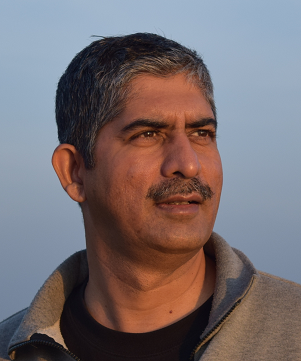
\includegraphics[width=0.8\linewidth,keepaspectratio]{myphoto}
% \end{center}	  
\end{frame}


%%%%%%%%%%%%%%%%%%%%%%%%%%%%%%%%%%%%%%%%%%%%%%%%%%%%%%%%%%%
\begin{frame}[fragile]\frametitle{Sample Two Columns Slide}
\begin{columns}
    \begin{column}[T]{0.6\linewidth}
      \begin{itemize}
		\item aaa
	  \end{itemize}

    \end{column}
    \begin{column}[T]{0.4\linewidth}
      \begin{itemize}
		\item bbb
	  \end{itemize}
    \end{column}
  \end{columns}
\end{frame}

%%%%%%%%%%%%%%%%%%%%%%%%%%%%%%%%%%%%%%%%%%%%%%%%%%%%%%%%%%%%%%%%%%%%%%%%%%%
\begin{frame}[fragile]\frametitle{References}
\begin{itemize}
\item Lessons from Fireside chat by Nassim Nicholas Taleb and Naval Ravikant
- Ravi Ranjan
\end{itemize}
\end{frame}